\documentclass[
	12pt,				% tamanho da fonte
    oneside,			% Oposto a twoside
	a4paper,			% tamanho do papel.
	english,			% idioma adicional para hifenização
	french,				% idioma adicional para hifenização
	spanish,			% idioma adicional para hifenização
	brazil				% o último idioma é o principal do documento
	]{abntex2}

\usepackage{lmodern}			% Usa a fonte Latin Modern			
\usepackage[T1]{fontenc}		% Selecao de codigos de fonte.
\usepackage[utf8]{inputenc}		% Codificacao do documento (conversão automática dos acentos)
\usepackage{lastpage}			% Usado pela Ficha catalográfica
\usepackage{indentfirst}		% Indenta o primeiro parágrafo de cada seção.
\usepackage{color}				% Controle das cores
\usepackage{graphicx}			% Inclusão de gráficos
\usepackage{microtype} 			% para melhorias de justificação
\usepackage{float} 			    % para fixação de imagens
\usepackage{caption}
\usepackage{lipsum}				% para geração de dummy text

\usepackage[brazilian,hyperpageref]{backref}	 % Paginas com as citações na bibl
\usepackage[alf]{abntex2cite}	% Citações padrão ABNT

\newcommand{\dd}[1]{\mathrm{d}#1}

% Pacote para a definição de novas cores
\usepackage{xcolor}
% Definindo novas cores
\definecolor{verde}{rgb}{0.25,0.5,0.35}
\definecolor{jpurple}{rgb}{0.5,0,0.35}
\definecolor{darkgreen}{rgb}{0.0, 0.2, 0.13}
% Configurando layout para mostrar codigos Java
\usepackage{listings}

\newcommand{\estiloC}{
\lstset{
    language=C,
    basicstyle=\ttfamily\small,
    keywordstyle=\color{jpurple}\bfseries,
    stringstyle=\color{red},
    commentstyle=\color{verde},
    morecomment=[s][\color{blue}]{/**}{*/},
    extendedchars=true,
    showspaces=false,
    showstringspaces=false,
    numbers=left,
    numberstyle=\tiny,
    breaklines=true,
    backgroundcolor=\color{cyan!10},
    breakautoindent=true,
    captionpos=b,
    xleftmargin=0pt,
    tabsize=2
}}

% ---
% Informações de dados para CAPA e FOLHA DE ROSTO
% ---
\titulo{Relatório de Estágio}
\autor{Felipe Marinho Tavares}
\data{Dezembro de 2018}
\local{Campinas -- São Paulo -- Brasil}
\instituicao{%
  Empresa: SAMSUNG ELETRÔNICA DA AMAZÔNIA
  \par
  Setor: Artificial Intelligence Research \& Development
  \par\par
  Supervisor: Ciro Cavani
  \par
  Orientador: Juliano de Almeida Monte-Mor
  \par\par
  Engenharia de Computação
  \par
  Universidade Federal de Itajubá -- UNIFEI
  }
\tipotrabalho{Relatório de Estágio}
% O preambulo deve conter o tipo do trabalho, o objetivo,
% o nome da instituição e a área de concentração
% ---

% ---
% Configurações de aparência do PDF final

% alterando o aspecto da cor azul
\definecolor{blue}{RGB}{41,5,195}

% informações do PDF
\makeatletter
\hypersetup{
     	%pagebackref=true,
		pdftitle={\@title},
		pdfauthor={\@author},
    	pdfsubject={\imprimirpreambulo},
	    pdfcreator={LaTeX with abnTeX2},
		pdfkeywords={abnt}{latex}{abntex}{abntex2}{trabalho acadêmico},
		colorlinks=true,       		% false: boxed links; true: colored links
    	linkcolor=blue,          	% color of internal links
    	citecolor=blue,        		% color of links to bibliography
    	filecolor=magenta,      		% color of file links
		urlcolor=blue,
		bookmarksdepth=4
}
\makeatother
% ---

% ---
% Espaçamentos entre linhas e parágrafos
% ---

% O tamanho do parágrafo é dado por:
\setlength{\parindent}{1.3cm}

% Controle do espaçamento entre um parágrafo e outro:
\setlength{\parskip}{0.2cm}  % tente também \onelineskip

% ---
% compila o indice
% ---
\makeindex
% ---

% ----
% Início do documento
% ----
\begin{document}

% Seleciona o idioma do documento (conforme pacotes do babel)
%\selectlanguage{english}
\selectlanguage{brazil}

% Retira espaço extra obsoleto entre as frases.
\frenchspacing

% ----------------------------------------------------------
% ELEMENTOS PRÉ-TEXTUAIS
% ----------------------------------------------------------
% Capa e Folha de Rosto
\imprimircapa
\imprimirfolhaderosto*
% ---

% ---
% inserir o sumario
% ---
\pdfbookmark[0]{\contentsname}{toc}
\tableofcontents*
\clearpage
% ---

% ----------------------------------------------------------
% ELEMENTOS TEXTUAIS
% ----------------------------------------------------------
\textual

% ----------------------------------------------------------------
% Introdução e Conceitos Básicos *******************
% ----------------------------------------------------------------
\chapter{Introdução}

Este relatório de estágio busca descrever o período de estágio de 16/04/2018 à 31/12/2018 na empresa SAMSUNG ELETRÔNICA DA AMAZÔNIA. O estágio supervisionado é componente curricular obrigatório junto à Universidade Federal de Itajubá. No curso de Engenharia de Computação, a carga horária necessária é de 196 horas.

O aluno atua na área intitulada Samsung Research Brazil (SRBR), foto na \autoref{fig:SRBR}, fazendo parte do time de Artificial Intelligence Research \& Development (AI R\&D).

\begin{figure}[H]
  \centering
  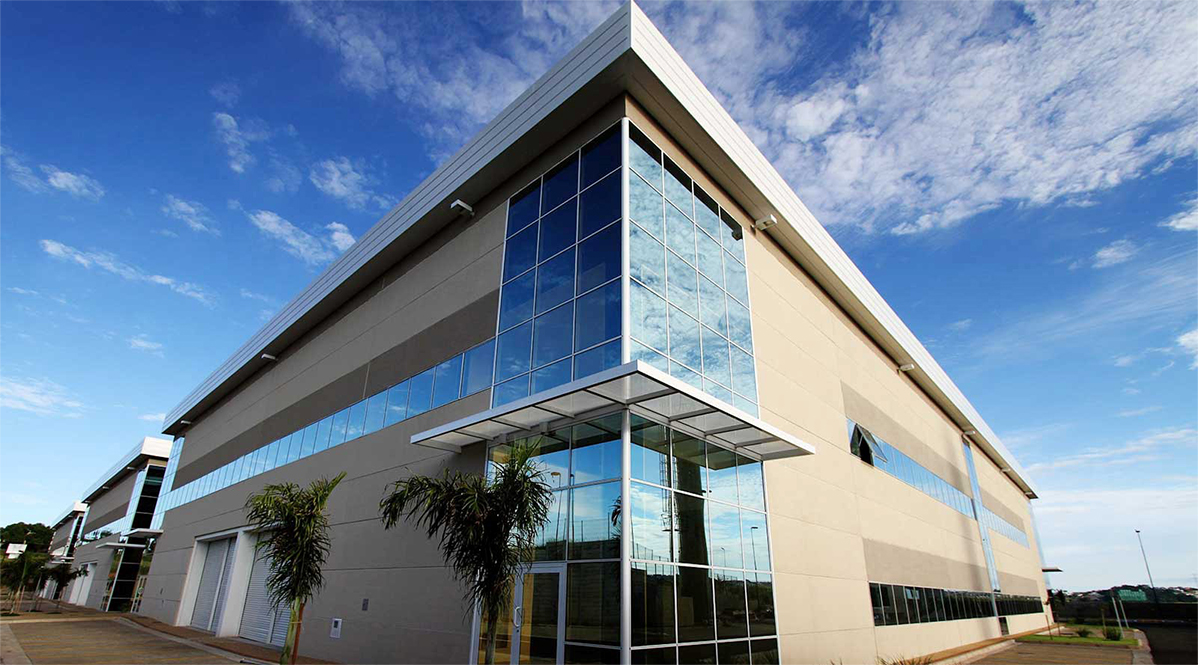
\includegraphics[width=400pt]{Imgs/srbr-image.jpg}\\
  \caption[SRBR, Samsung Research Brazil]{SRBR, Samsung Research Brazil}
  \label{fig:SRBR}
\end{figure}

A NXP opera no Brasil junto ao BSTC, ou Brazilian Semiconductor Technology Center, dentro do complexo Technopark em Campinas, São Paulo. Suas instalações permitem o desenvolvimento de \textit{chips} e microcontroladores que são, então, produzidos e distribuídos ao redor do mundo.

O modelo de contrato firmado entre a NXP e a universidade foi firmado tendo o o CIEE como intermediário. Segundo \citeauthor{Cartilha}, esse órgão, de nome "Centro de Integração Empresa-Escola", é considerado um agente de integração, e tem por responsabilidade fazer o acompanhamento administrativo das oportunidades de estágio no estado de São Paulo.

Desde o início do processo, diversas atividades foram desenvolvidas, auxiliando projetos dentro da empresa e permitindo crescimento pessoal e profissional. A NXP fabrica produtos na linha de \textit{chips} semicondutores para utilização de terceiros. Assim sendo, as atividades auxiliaram na criação desse tipo de produto, sendo efetivas como modo de ensino e tendo resultados práticos, observáveis no fluxo de trabalho da empresa.

Dessa maneira, o estágio cumpriu os objetivos firmados até presente momento. Tais objetivos são três, e serão discutidos a seguir.

\section{Contexto e Objetivos}

A NXP é uma empresa com notáveis produtos na área de tecnologia, especificamente em microprocessadores e microcontroladores. Dessa forma, a área de atuação da empresa é compatível com matérias observadas durante a grade curricular. Matérias como Eletrônica Digital I e II, Eletrônica Analógica I e II, Circuitos Integrados Digitais, Computadores Digitais e Microcontroladores I e II sumarizam os conhecimentos iniciais necessários que seja possível trabalhar com conceitos desenvolvidos dentro da empresa.

Dessa maneira, o primeiro objetivo tido para o processo é o promovido pela própria universidade, que é o de integrar o educando ao ambiente de trabalho e desenvolver habilidades específicas mais comumente utilizadas na indústria.

O segundo objetivo, de cunho pessoal, é o de devolver todo o investimento à empresa na forma de resultados. Isso se dá pois, para todo novo tipo de conhecimento, é necessário treinamento para que se atinja a excelência. No ambiente acadêmico, faz parte da grade de atividade dos professores ensinarem seus alunos acerca das atividades desenvolvidas. Numa empresa de pequeno a grande porte, entretanto, é preciso que sejam alocados recursos de outras áreas para que se efetue um treinamento adequado. 

Dessa maneira, o segundo objetivo para o processo de estágio é o de trabalhar em atividades que complementem o fluxo da empresa, adicionando à força de trabalho do restante do grupo.

A área de comportamento e habilidades de comunicação e interpessoais não é normalmente desenvolvida durante os cursos acadêmicos, sendo deixada como aprendizado pessoal ou através de cursos de extensão. Esse tipo de habilidade vem, cada vez mais, sendo valorizada no âmbito profissional, já fazendo parte de processos seletivos como característica desejada nos profissionais. Assim sendo, por fim, objetiva-se analisar e aprender sobre as habilidades comportamentais requeridas na empresa para que o ambiente de trabalho se torne o mais agradável e produtivo possível. 

Com esses três objetivos, espera-se que companheiros de trabalho e empresa gerem um retorno positivo a cerca das atividades exercidas, assim como pelo comportamento durante o estágio. Dessa forma,todos se beneficiariam mutuamente, reforçando o objetivo principal do processo.

% ----------------------------------------------------------------
% Introdução e Conceitos Básicos *******************
% ----------------------------------------------------------------
\chapter{Revisão Bibliográfica}

\section{História}

Freescale e NXP são, hoje, uma só empresa que atua no mercado de microcontroladores. No entanto, cada uma delas teve uma trajetória distinta até se tornarem o que são atualmente.

\subsection{Freescale}

A Freescale era, originalmente, uma divisão de semicondutores, criada em 1948 por sua empresa originária, Motorola. Como uma das primeiras empresas no setor, a Motorola foi de extrema importância para o programa espacial dos Estados Unidos durante a corrida espacial e os Programas Apollo, fornecendo diversos materiais e equipamentos para as missões. Inicialmente voltada para Radiofrequência e Comunicações, a divisão eventualmente se voltou para o desenvolvimento comercial de produtos para o mercado automotivo e de semicondutores.


A partir desse crescimento constante e pelos crescentes lançamentos pioneiros no mercado, a Motorola anunciou, em 2003, que a divisão de semicondutores seria oficialmente separada para a criação da Freescale. Já como empresa independente, novas linhas de produtos e melhorias foram apresentadas, tornando a empresa influente em setores como geração de energia solar e embarcados na medicina. Também foram criados os produtos da linha Kinetis, considerados à época os menores \textit{chips} ARM do mundo, rivalizando os \textit{chips} oferecidos pela líder no setor, Atmel. 

\subsection{NXP}

A NXP foi, inicialmente, criada como um setor de pesquisa da empresa Phillips, em 1953, com o nome oficial de Phillips Semiconductors. Esse setor recebeu aquisições importantes, como a Signetics, responsável pela criação do temporizador 555, e a VLSI Technology. O setor de semicondutores da empresa se destacou, também, pela criação de tecnologias inovadoras e ímpares no mercado, como o NFC e \textit{chips} de identificação utilizados em passaportes.

Em 2006, o setor de semicondutores se separou de sua matriz, Phillips, tomando para si o novo nome de NXP. Essa transação foi feita pela compra de 80.1\% do setor de semicondutores por um consórcio de investidores, fazendo parte desse consórcio grupos como Kohlberg Kravis Roberts(KKR), Bain Capital, Silver Lake Partners, Apax Partners e AlpInvest Partners.



Já então como NXP, a empresa adquiriu companhias independentes ao longo de sua trajetória que poderiam auxiliar na expansão de novas áreas de mercado, assim como no estudo de novas tecnologias que estivessem se destacando dentre as já disponíveis. Dessa maneira, suas aquisições começaram já no início de sua separação, em 2007, com a AeroFONE, e se seguiram nos anos seguintes, variando desde \textit{joint ventures} até processos de restruturações e compra de empresas estratégicas para sua própria expansão.

Finalmente, em 2015, foi anunciado o acordo de fusão entre a NXP e Freescale, sendo a NXP a compradora. A partir deste ponto, todos os recursos pertencentes à Freescale se tornaram parte da NXP.

Como sua missão principal, a NXP preza por criar a infraestrutura e as conexões seguras que permitirão um mundo mais inteligente, criando assim soluções que tornem as vidas de pessoas mais fáceis, melhores e mais seguras.

\section{Semicondutor}

Um material semicondutor, de acordo com \citeauthor{Holger}, é capaz de conduzir corrente dependendo de diferentes condições ambientais e de dopagem de seu material. Dessa maneira, controlando essas condições, é possível conduzir uma quantidade espeífica corrente através de um circuito e acionar mecanismos de maneira controlada. Uma das condições possíveis de se controlar é o estado elétrico de um componente. Um diodo, segundo \citeauthor{Umesh} e \citeauthor{Amos}, é capaz de conduzir corrente quando o sentido desta segue de acordo com sua polarização, como representado na Figura \ref{fig:DIODO}. Caso o ânodo a receba, o diodo se torna transparente e o circuito pode ser simplificado como fechado. Já no caso em que o ânodo recebe corrente, o diodo não conduz e o circuito pode ser simplificado como aberto.



Estruturas mais complexas, como o transistor, permitiram o desenvolvimento de sistemas muito mais efetivos e controlados que aqueles possibilitados por diodos. Ainda conforme \citeauthor{Amos}, o transistor funciona de maneira análoga, porém com quatro terminais. Um deles representa a entrada de corrente, chamado de Fonte ou Source, e o outro a saída, denominado Dreno ou Drain. O maior diferencial é um terminal de controle, chamado de Porta ou \textit{Gate}. Ele funciona como uma chave que determina se a corrente será ou não transmitida pelo transistor. Caso seja alimentado, o \textit{Gate} permite a passagem, não a permitindo no caso oposto. Finalmente, existe um outro terminal chamado de Substrato, que costuma ser ligado em curto-circuito com a fonte e tem funcionalidades específicas para transistores mais sofisticados. A maneira com que esses terminais estão dispostos no transistor pode ser observada na Figura \ref{fig:NMOS}.



A partir desse novo nível de controle, eventualmente foi descoberto que, utilizando um conjunto de transistores, era possível codificar uma linguagem baseado no seu estado elétrico. Essa codificação foi regida por diretrizes que determinavam que o sinal pode ser representado de maneira binária, com os valores 0 ou 1, que dependem da intensidade da corrente através do fio num dado momento. Estabelecida essa representação de dados, que é diretamente ligada ao estado de "ligado" ou "desligado", foi possível então aplicar estruturas de tratamento e transmiti-los de maneira controlada através de um circuito. A partir disso, por fim, geraram-se dados num componente, sendo estes transmitidos de maneira compreensível para outros, que os utilizariam nas suas próprias funções, aumentando exponencialmente a gama de aplicações eletrônicas que poderiam ser desenvolvidas para o mercado.

\section{Clock}

A estrutura de base de tempo dentro de um \textit{chip} é denominada \textit{clock}, e, conforme \citeauthor{Masami}, consiste num gerador que varia na frequência de, por exemplo, um cristal oscilatório, como demonstrado na Figura \ref{fig:OSC}. Esse gerador opera em determinada frequência e sua saída é transmitida para diversos componentes do sistema, para que eles possam então funcionar de maneira síncrona. Um sistema permite a utilização de vários \textit{clocks}, porém é necessário cuidado para que processos em grupos de componentes envolvendo diferentes \textit{clocks} levem em conta riscos de dessincronização, e atuem com lógica especial para preveni-los.



A estrutura básica de armazenagem de dados num \textit{chip} é denominada \textit{Flip-flop}, e seu funcionamento, segundo \citeauthor{Mano}, é dado através de portas dispostas de maneira a permitir a passagem de dados de maneira intercalada. Dessa maneira, é possível alimentar o componente com um dado e, após um ciclo de \textit{clock}, ele será propagado no circuito. Essa estrutura é uma das mais importantes na construção de componentes eletrônicos, sendo vital em qualquer aplicação que requeira controle sob os dados sendo transmitidos em seus terminais.


A estrutura interna do \textit{Flip-flop} mais utilizado, o tipo D, consiste nos componentes primitivos observados na figura \ref{fig:FLIPFLOPD}. Duas entradas, uma de dados e outra de controle, normalmente o \textit{clock}, inserem no componente os dados necessários para que o \textit{flop} possa transmitir a informação de maneira sincronizada. Na primeira borda de subida de E, o valor em D é propagado normalmente e inversamente para os terminais de saída, e tais valores são mantidos enquanto o \textit{clock} não recebe outra borda de subida. As quatro portas NAND representam dois latches tipo D trabalhando em conjunto, que são estruturas mais simples que o \textit{flop} que não requerem sinal de controle para seu funcionamento. Unindo-se as duas, é possível controlar melhor o comportamento do dispositivo pela adição do segundo sinal de entrada.

\section{SoC}

Uma das aplicações tornada possível desde o desenvolvimento da tecnologia de transistores foi a de \textit{chips} capazes de computar dados e os distribuir através de suas conexões periféricas. Esses produtos, em geral, comportam de milhares a milhões de transistores dentro de seus circuitos. 

Os produtos chamados \textit{SoC}, ou \textit{System on Chip}, são componentes eletrônicos complexos que, segundo \citeauthor{Flynn}, envolvem processadores, memórias e interconexões criadas para um certo campo de aplicação. A gama de aplicações que eles podem suportar é virtualmente infinita, dependendo apenas do seu processo de fabricação e para o quê o \textit{chip} foi projetado. Aplicações mais utilizadas costumam ser digitais, analógicas, mistas analógico-digitais e em rádio frequência. Eles também são vastamente utilizados no mercado de embarcados, sendo, usualmente, o componente principal da aplicação, agindo como controlador ou o processador de outros componentes.

O desenvolvimento de um \textit{SoC} passa por várias etapas antes de chegar até o consumidor final, desde a análise financeira do projeto, diversas etapas de criação do \textit{chip} até análises de qualidade. Para que seja possível analisar esse processo, é necessário primeiro estudar os vários conceitos importantes que ditam seu processo de criação.

\section{Timing}

Circuitos são, em termos microeletrônicos, grandes. Portanto, durante a alimentação de todos os componentes com os \textit{clocks} do circuito, é normal que sinais provenientes do mesmo \textit{clock} atinjam diferentes componentes com diferentes fases, determinadas pela quantidade de atraso presente num caminho. É comum que esses diferentes componentes compartilhem um caminho de dados entre si, o que pode acarretar em diversas violações que impactam diretamente no funcionamento e nos processos de simulação de um \textit{chip}.

Para combater esses atrasos, a etapa de \textit{Timing} é, de acordo com \citeauthor{Sridhar}, onde a sincronia entre os componentes do \textit{chip} é analisada. Caso a diferença de fase do sinal de \textit{clock} entre os componentes exceda um valor passado como parâmetro, são, então, feitos reparos no circuito até que os valores observados estejam dentro do desejado. O valor inicial passado depende de diferentes fatores que influenciam na interação entre diferentes componentes, baseado em seu \textit{clock}. O objetivo final é atingir a sincronia mais perfeita possível entre componentes, como observado na Figura \ref{fig:NOSHVIOL}.



Conforme \citeauthor{Bhasker}, Skew é o nome dado para o atraso quantificável do \textit{clock} entre dois ou mais componentes num circuito, como observado na Figura \ref{fig:SKEW}. Sendo um fenômeno observável apenas nos caminhos de \textit{clock}, não existe lógica implementada que possa influenciar o tempo de chegada ou de atraso além da colocada propositalmente para controle. A lógica presente não afetando o valor de \textit{skew}, o fator mais influente no atraso é a capacitância interna aos fios, provocada pelas distâncias de propagação entre o sistema que produz o \textit{clock} e o componente que o recebe. Para mitigar os problemas de temporização, são utilizados componentes chamados \textit{buffers} e inversores, que atuam como atrasos controlados no caminho de \textit{clock} até o componente. Normalmente, são atribuídos valores máximos suportáveis num projeto sem que o \textit{chip} apresente problemas de funcionamento. Em todo caso, é sempre desejado que se atinja o valor ótimo, zero.

\subsection{Slew}

\textit{Slew} é uma aproximação do comportamento real de sinais dentro de um \textit{chip}. Isto é, é uma representação mais fiel, dentro de simulações, de como o sinal vai se comportar, assim evitando possíveis problemas devido ao modelo utilizado não ser compatível com seu funcionamento real. De acordo com \citeauthor{Bakshi}, o efeito consiste no fato de que o sinal não vai do valor 0 ao 1, ou 1 ao 0, instantaneamente, mas sim durante um período de transição. Nesse período, é importante que outros componentes sejam mantidos em espera até que o sinal se normalize, de modo a garantir uma transmissão correta dos dados. Essa transição pode ser observada na figura \ref{fig:SLEW}. A transição de 0 a 1 é sempre mais rápida que a de 1 a 0, devido ao funcionamento dos transistores utilizados nos componentes.



\subsection{Metaestabilidade}

Metaestabilidade é, segundo \citeauthor{Ben}, o fenômeno onde a intensidade do sinal varia entre os limites interpretados como 0 ou 1 na entrada ou saída de um componente. Esse fenômeno ocorre quando dois \textit{flops}, de diferentes \textit{clocks}, estão propagando um dado serialmente. O problema ocorre quando o \textit{clock} do segundo \textit{flop} ativa o processo de captura enquanto o primeiro está carregando o fio comum aos dois, fazendo com que a informação capturada esteja entre os valores de tensão característicos para 0 ou 1. Desta maneira, o primeiro \textit{flop} transmite o sinal normalmente, porém o segundo captura uma informação que não está, ainda, caracterizada, e sim em estado de metaestabilidade. Quanto isso ocorre, é impossível predizer o comportamento do circuito adiante à violação, o que impossibilita qualquer tipo de análise ou desenvolvimento.

Normalmente, garante-se que não há metaestabilidade entre componentes de diferentes \textit{clocks} quando é empregado um conjunto de sincronizadores. Tais componentes são compostos de dois ou mais \textit{flip-flops} em série, que utilizam um número equivalente de ciclos de \textit{clock} para normalizar o valor capturado do sinal ao fim da série, e então propagar o dado de maneira correta.



Conforme observado na figura \ref{fig:MSVIOL}, os diferentes \textit{clocks} entre os \textit{flops} provocam a captura, no segundo \textit{flop}, do sinal ainda em estado de transição. Isso faz com que o valor observado no terminal Q2 do \textit{flop} 2 não possua valor estável, indicado na imagem no círculo vermelho, gerando um valor simulado de "X", ou metaestabilidade, em ferramentas como \textit{NCVerilog} ou \textit{Tessent}, e comportamento imprevisível em \textit{chips} e circuitos físicos.

\subsection{Setup Hold}

Um dos fatores que mais provocam falhas de \textit{timing} ao longo do projeto são violações de \textit{Setup-Hold} entre componentes. Essas violações ocorrem devido a quantidade de atraso provocada pela lógica presente, ou até mesmo pela capacitância intrínseca aos fios, que aumenta diretamente proporcionalmente á sua distância. O atraso pode ser muito pequeno ou muito grande, fazendo com que o dado seja propagado no fio de maneira a atingir o próximo terminal fora da faixa aceitável, indicando que é possível que se ocorram violações. Para tratar destes erros, normalmente é necessário alterar a lógica de dados a fim de aumentar sua velocidade, ou ainda o mais comum, que é incluir lógica de atraso dentro dos caminhos de \textit{clock}, a fim de que os componentes se tornem sincronizados levando em conta os atrasos adjacentes.

A violação de \textit{setup} ocorre, de acordo com \citeauthor{Wang}, quando o dado propagado entre o primeiro \textit{flop} não consegue atingir o segundo a tempo de ser transmitido pela borda de subida do \textit{clock} comum aos dois. Dessa maneira, o segundo \textit{flop} propaga a informação anterior duas vezes antes de passar para a próxima, efetivamente ignorando a informação recente e criando um chamado \textit{mismatch}, que é um valor diferente do inicialmente transmitido. O tempo de \textit{setup} indica o tempo necessário para que o dado na entrada do \textit{flop} esteja estável, para que tal dispositivo consiga, então, propagá-lo de maneira adequada através do circuito. 



Como pode ser observado na figura \ref{fig:SVIOL}, o dado propagado através do primeiro \textit{flop}, do terminal D1 para Q1, atinge o terminal D2 do segundo \textit{flop} muito depois do período de captura, dado pela subida do \textit{clock}, marcada verticalmente em vermelho claro. Assim sendo, o valor propagado para o terminal Q2 difere do esperado para o conjunto. Isso normalmente se deve pela lógica encontrada entre o caminho de dados entre os dois \textit{clocks}.

Segundo \citeauthor{Greg}, a violação de hold ocorre na situação oposta. Isto é, quando a informação entre os componentes é passada de modo tão rápido que o \textit{clock} não perfeitamente sincronizado do segundo componente não consegue capturar o dado corretamente. Assim, a saída do segundo \textit{flop} captura o primeiro e o terceiro dados, não observando o segundo durante o período de subida de seu \textit{clock}. Para evitar tal situação, é necessário um tempo de \textit{hold}, que se refere, justamente, ao tempo que o componente mantém o dado recebido em seu circuito para propagação, para que não ocorra a violação onde o dado correto é sobrescrito pelo o que vem próximo na fila.



De acordo com a figura \ref{fig:HVIOL}, o dado, ao sair do terminal Q1, atinge o terminal D2 quase que instantaneamente, não sendo capturado a tempo pela borda de subida de clk2. Dessa maneira, o dado propagado para Q2 não é o corrente, mas sim o próximo. Como a função do sinal em D1 é sempre igual, pode-se observar que seu resultado em Q2 é invertido. Isso não se mantém, porém, para simulações onde os valores de sinal não sejam sempre sabidos, e muito menos em um \textit{chip} físico, onde seu comportamento será errático e o funcionamento do sistema poderá sofrer falhas graves devido á transmissão incorreta de sinais.

\section{Fluxo de Projeto}

O processo de criação de um \textit{chip} é longo e envolve uma grande quantidade de profissionais, cada um especializado numa diferente etapa. Dentro deste processo, várias etapas acabam sendo classificadas sob identificadores, que auxiliam os gerentes e líderes de times determinar mais facilmente o estado de maturidade do projeto e poder estimar ações cabíveis para otimizar o ritmo de produção.

Tomando o maior escopo da produção, assim como o nível de abstração mais alto possível, é possível traçar um diagrama de todo o caminho de produção, representado na Figura \ref{fig:FLOWTOTAL}.



A primeira etapa no fluxo envolve a criação dos IPs, denominados \textit{Intellectual Properties}. Estes são componentes que possuem funcionalidades específicas no \textit{chip}. Naturalmente, para construir qualquer todo, é necessário que sejam desenvolvidas primeiro suas partes, e o desenvolvimento destas gera os IPs. Essa etapa envolve a criação tanto de IPs digitais quanto analógicos, podendo existir, entretanto, IPs que possuem componentes digitais e analógicos funcionando em sincronia. Como normalmente o desenvolvimento desses IPs Digitais-Analógicos termina na parte Digital, o fluxo de desenvolvimento divide as duas partes e as coloca na ordem vista na Figura \ref{fig:FLOWTOTAL}.



Segundo \citeauthor{Bakshi2}, a principal diferença entre IPs digitais e analógicos é a maneira com que seus sinais são tratados. Como visto na Figura \ref{fig:ADIP}, IPs analógicos trabalham com sinais reais, com variações ocorrendo através do tempo contínuo. Nessa forma, o sinal possui o máximo de fidelidade com o mundo real, ao custo de apresentar muito maior dificuldade no seu tratamento e utilização. Já em IPs digitais, o sinal é obtido periodicamente, oferecendo um sinal com representação aproximada à real, porém com controle e velocidades de operação muito maiores.

\subsection{Analog IP}

IPs analógicos são as estruturas que tem funcionalidades específicas que ferramentas são incapazes de gerar de forma digital. Dessa forma, essa etapa requer desenvolvimento a nível de transistores e estudos dos vários limites eletrônicos para o componente, afim de que atendam o necessário para a aplicação para qual estão sendo desenvolvidos. Estes limites são geralmente a tensão, corrente, capacitância e impedância.

\subsection{Digital IP}

IPs digitais são sintetizáveis por ferramentas a partir de linguagens descritivas. Isso indica que sua construção é possível a partir de estruturas lógicas básicas, como portas AND, OR, XOR, NAND e NOT. Dessa maneira, linguagens como Verilog, VHDL ou ainda SystemVerilog são normalmente as utilizadas no processo de construção destes componentes. Em casos de IPs analógicos mais complexos, é geralmente necessária a criação de uma interface digital para que possa existir uma comunicação mais eficiente entre o IP e o resto do \textit{chip}. Para tal, os times responsáveis comunicam entre si para compartilhar as especificações desejadas e trabalhar na criação do componente.

\subsection{Integration}

Uma vez criada a lista de componentes e a plataforma de colaboração, é possível prosseguir para a etapa de Integração. Nessa, IPs são conectados entre si e sua funcionalidade é aplicada de maneira a funcionar de modo harmonioso. Dependendo dos IPs conectados, e da maneira que o são, é possível gerar funcionalidades mais complexas e produzir um \textit{chip} com características específicas, como maior potência, menor consumo ou menor \textit{leakage}. Junto a essa conexão, é necessário distribuir os componentes no espaço físico destinado ao \textit{chip}, tomando cuidado com as posições de cada IP para que as conexões não excedam distâncias muito grandes, o que geraria problemas de sincronismo no sistema.

É ao fim da etapa que ocorre o \textit{Tape Out}, isto é, o projeto sai do âmbito virtual e passa para o real, com a produção do silício contendo o \textit{chip}. A partir desse ponto, é então possível verificar o controle de qualidade ao promover testes e análises que vão observar o comportamento do produto num ambiente real, e não simulado.

\subsection{Testing}

Já, então, com o \textit{chip} fisicamente disponível, a etapa de teste consiste em verificar que padrões e rotinas, geradas na etapa de integração, retornem resultados positivos quando exercitadas. Segundo \citeauthor{Krishnendu}, a maneira com que esses testes acontecem é através de máquinas especialmente desenvolvidas, chamados testadores, para exercitar os pinos do \textit{chip}. Elas possuem agulhas ou sockets, produzidos especificamente para cada modelo de \textit{chip}, e são, então, programadas para gerar valores iguais aos dos padrões, testando a funcionalidade da parte lógica e verificando se existe algum tipo de erro gerado pela má produção do \textit{chip}.

\subsection{Validation}

Finalmente, a etapa de validação é responsável por conduzir análises no \textit{chip} que confirmem suas características determinadas ao longo do projeto. Além de confirmar via testes de bancada, que são estímulos e medições com aparelhos de laboratório em placas de teste que contém o chip, que ele funciona, é interessante também exercitar o \textit{chip} com valores máximos de forma a verificar seus limites de atuação.

\subsection{Verification}

Além do fluxo normal de produção de um \textit{chip}, é necessário também garantir que não haja erros ao longo do projeto. Um erro que se propague sem controle traria prejuízos não mensuráveis ao produto final e à empresa. Dessa maneira, existem divisões responsáveis por verificar as atividades dos outros times, através das diferentes etapas do projeto. No caso do grupo de verificação, cada modificação feita em IPs individuais requer a ação de um verificador para garantir que o componente mantém a funcionalidade descrita em sua especificação. De maneira análoga, é necessário um time de verificação para testar, também, modificações feitas ao código do \textit{chip}. Essa última ocorre na etapa de integração, para confirmar que as ligações continuam funcionais e que é possível transmitir informação apropriadamente através de componentes. Dessa maneira, o grupo de verificação começa seu trabalho já no início da vida de um projeto, e continua ativamente até o momento em que não houver mais nenhuma alteração física ou lógica no \textit{chip}.

\subsection{DFT}

Segundo \citeauthor{Laung}, a etapa de DFT, sigla para \textit{Design for Testability}, é responsável por adicionar, principalmente durante a integração, componentes e lógica no \textit{chip} que permitam que o time de testes efetue, nas etapas futuras, testes que proporcionem ao projeto a maior taxa de cobertura possível. Ao testar o \textit{chip}, é possível detectar discrepâncias entre a lógica e o físico. assim promovendo maior segurança e qualidade para o projeto.

Esse grupo é considerado parte do grupo de Integração, devido às atividades desenvolvidas e ao período de atuação da equipe. Sua representação única no fluxo se faz necessária, entretanto, por sua atuação persistir após o \textit{Tape Out}, continuando durante o período de testes. Nessa nova fase, geralmente existe a geração de novos padrões para melhor cobertura ou eventual análise do RTL para correções. Uma testabilidade eficiente garante que problemas de fabricação sejam detectados e que a peça defeituosa seja descartada antes de chegar ao cliente.

\section{Integração}

A etapa de integração é a maior no que diz respeito ao desenvolvimento do projeto já definido. Isto é, as etapas iniciais vistas anteriormente referentes a IP digital e analógico geralmente acontecem sem o objetivo de atender a um \textit{chip} específico, mas sim de adentrarem uma lista de materiais que possam ser utilizados em múltiplos projetos no futuro. Assim, num projeto, é incomum que as etapas iniciais promovam o desenvolvimento de novos IPs, mas sim que sejam escolhidos os mais atualizados e apropriados para o projeto a ser desenvolvido.

Dessa maneira, sendo a maior etapa, o fluxo de integração possui diversos passos internos que garantem o bom funcionamento do \textit{chip}. Esses passos estão todos demonstrados na Figura \ref{fig:FLOWINT}. Conforme já indicado, qualquer alteração nessa etapa passa pela verificação, o que significa que qualquer alteração em RTL, independente do passo, necessita da aprovação de um verificador para seguir para o \textit{Tape Out}.



\subsection{Specification}

O passo inicial da integração consiste em reforçar as especificações do projeto e consolidar características chave, de maneira a evitar que grandes alterações sejam propostas ou colocadas em etapas mais avançadas, quando implementá-las já não é viável do ponto de vista financeiro. Isso se deve ao fato de que, geralmente, quanto mais próximo do \textit{Tape Out} uma alteração ocorre, mais etapas necessitam ser revisitadas para que ela ocorra com qualidade e sem a possibilidade de falhas. Isso acaba acarretando em grandes custos adicionais ao projeto que poderiam ser evitados, caso houvesse uma definição mais concreta e final já ao começo do fluxo.

\subsection{RTL e Placement}

A partir desse ponto, onde todos os blocos de componentes já estão apropriadamente determinados, é iniciado o processo de criação do \textit{chip} descritivamente e fisicamente. Essa parte normalmente se inicia através de modificações em RTL, ou \textit{Register Transfer Language}, seja a partir apenas das especificações de componentes e funcionalidades ou de um \textit{chip} já existente. Suficientemente especificado, é possível começar a projetar e simular a disposição dos componentes no espaço físico e dispor as diversas portas lógicas do netlist na área reservada ao chamado \textit{Sea of Gates}, que é a área que contém a lógica geral do circuito. Toda essa disposição se dá através de ferramentas de posicionamento como a representada em \ref{fig:CHIP}. Nessa etapa também é adicionada uma versão preliminar das ligações entre componentes, sem levar em conta regras de posicionamento e da tecnologia utilizada, assim como os trilhos referentes a alimentação, compostos de \textit{VSS} e \textit{VDD}, que são os terminais negativos e positivos do \textit{chip}, respectivamente.



Geralmente, a etapa de integração de RTL, sozinha, toma uma enorme porcentagem do projeto, devido à eventuais mudanças de especificação não previstas, alterações feitas a componentes devido a demandas de clientes e erros que necessitam de reparos ao longo do projeto. É comum essa etapa se estender por meses e andar paralela a outras atividades, sendo distribuída nas chamadas \textit{builds} ou \textit{releases}, que podem acontecer periodicamente ou a critério do gerente de projeto.

\subsection{Synthesis}

Após completadas todas as mudanças em \textit{RTL} esperadas no projeto, o gerente assinala o início do processo de síntese, que consiste em pegar todo o código em \textit{RTL} criado através dos processos anteriores e o converter, através de ferramentas, num código único que descreve o \textit{chip}. Essa descrição difere da criada anteriormente por estar condensada num único arquivo, chamado de \textit{netlist}, além de conter novos componentes que aproximam a descrição do \textit{chip} da realidade, como \textit{buffers} e \textit{flops} para transmissão apropriada dos dados.

Esses componentes, gerados automaticamente, são escolhidos a partir de uma gama de opções selecionadas pela pessoa responsável pela sintetização. Essas opções são denominadas \textit{constraints} e são escolhidas para cada componente básico que o \textit{chip} utilize, como \textit{clocks} e fontes de alimentação. Elas determinam informações como o \textit{timing} dos componentes ou seu comportamento no \textit{chip}. Dessa maneira, a parte de escolher as \textit{constraints} costuma ser a mais custosa quanto a todo o processo de síntese.

Ainda na etapa de síntese, é colocada também a parte referente a \textit{DFT}, que consiste de \textit{constraints} específicos e todos os componentes necessários para tornar o \textit{chip} o mais testável possível. Assim, \textit{flops} são inseridos em cadeias a fim de que seja possível inserir valores de maneira controlada e observável. Caso não houvesse essa junção entre os dois processos de síntese, muitos pontos no \textit{chip} se tornariam pontos cegos, o que ocasionaria uma baixa cobertura, não atingindo as metas de qualidade esperadas.

Nessa etapa se inicia também, assim que surgirem as primeiras versões de \textit{netlist}, o processo de ATPG do grupo de DFT. Esse processo significa \textit{Automatic Test Pattern Generation} e consiste no emprego de uma ferramenta que criará todos os caminhos de teste, observáveis no circuito, de maneira automática. Nessa etapa, cabe ao operador rodar a ferramenta e corrigir o código de \textit{setup}, com \textit{constraints} e regras, a medida em que erros aparecerem. Em casos mais extremos, é necessário modificar o RTL para que maiores coberturas de ATPG sejam obtidas. Esse é um dos processos mais importantes para a etapa de DFT, dado que é o pacote de informações que será utilizado pelo time de testadores após a confecção do silício.

\subsection{CTS}

Com a versão final da síntese sendo lançada, é possível então proceder para a parte de CTS, sigla para \textit{Clock Tree Synthesis}. Conforme \citeauthor{Laung}, nessa etapa, várias ferramentas são utilizadas criar a chamada árvore de \textit{clocks}, como observado em \ref{fig:CTS}, para obter a diferença de latência entre os \textit{clocks} do \textit{chip} para cada componente, determinando assim o Skew e a necessidade de utilizar lógica para diminuir esse valor.



Uma vez criadas as árvores, são colocadas, então, todas as ligações entre \textit{clocks} e componentes, de maneira a se otimizar o circuito e evitar valores altos de \textit{skew}. Essa ligação envolve apenas o chamado \textit{timing path}, que é o caminho que gerencia o tempo de funcionamento nos dispositivos. O caminho responsável pela transferência de dados, chamado \textit{data path}, pode então ser adicionado na próxima etapa.

\subsection{Routing}

A etapa de \textit{Routing} é a última etapa de modificação das interconexões presentes no \textit{chip}, e envolve a colocação das conexões entre dispositivos levando em conta as regras de \textit{Design}, \textit{constraints} colocados no projeto e regras ou limitações impostas pela tecnologia utilizada. Essas ligações representam o \textit{data path} entre o circuito, permitindo que componentes troquem ou propaguem informação. Essa etapa é, também, responsável por distribuir essas conexões de maneira a otimizar a transmissão desses dados. Essa otimização acontece através de alguns procedimentos, como a remoção de gargalos, que acabam por aumentar a necessidade de alimentação da área e dificultar uma distribuição eficiente de energia, ou, ainda, aliviar constraints do circuito, de maneira que a ferramenta tenha maior liberdade de distribuir a conexões do sistema de maneira mais eficiente.

\subsection{Extraction e STA}

A etapa de extração acontece, por fim, depois do roteamento e da sincronização do \textit{chip} como um todo, e é responsável pela eliminação das capacitâncias parasitas existentes, a fim de que seja possível fazer análises reais de \textit{timing} do \textit{chip}. Uma vez obtidas essas análises, é possível então prosseguir para a etapa de \textit{STA}, ou \textit{Static Timing Analysis}. Essa etapa é uma das que mais consome tempo dentre todas, e tem importância enorme na garantia de que não existirá \textit{skew} nos componentes capaz de provocar mal funcionamentos por questões de violação de \textit{setup} ou de \textit{hold}. Segundo \citeauthor{Bhasker}, durante essa parte, são adicionados novos componentes de temporização no \textit{netlist}, como \textit{buffers} e inversores. Dessa maneira, o ponto de chegada dos sinais de \textit{clock} nos componentes é sincronizado em diversas áreas, de forma que não existam violações de tempo enquanto o \textit{chip} estiver funcionando.

\subsection{SI e DFM}

Uma vez que os erros de \textit{timing} são corrigidos, é possível então analisar características mais sutis do projeto nas próximas etapas, como em \textit{SI Analysis}, ou \textit{Signal Integrity Analysis}, onde uma nova análise leva em consideração as capacitâncias parasitas entre os metais de trilhos para detectar possíveis interferências danosas de sinais uns sobre os outros.

Junto ao \textit{SI} acontece também o \textit{DFM}, ou \textit{Design for Manufacturability}, onde algumas checagens são feitas para garantir uma melhor produção do \textit{chip}, com maior confiabilidade e menor necessidade de ajustes aos métodos de produção. Dessa maneira, custos de produção e chances de falhas no silício são reduzidas, o que acarreta em barateamento do processo de manufatura como um todo.

\subsection{LVS e DRC}

Implementadas otimizações de manufatura, o \textit{chip} está finalmente apto a ser produzido. Antes de ser despachado para as \textit{foundries} responsáveis pela produção, ele é então analisado mais uma vez através de uma etapa chamada \textit{LVS}, ou \textit{Layout Versus Schematic}, que checa possíveis diferenças entre o \textit{netlist} com a parte física. Garantida a equidade entre os dois modelos, são verificadas também a regras de Design, numa etapa denominada \textit{DRC}, ou \textit{Design Rule Checking}. Essas regras são estabelecidas durante a especificação, e são referentes às regras de Layout do chip. Algumas delas se referem à distância máxima entre os trilhos ou tamanhos máximos e mínimos para os dispositivos. Essas regras são definidas junto com a escolha da tecnologia a ser utilizada, e tem por objetivo garantir que não ocorram funcionamentos fora do esperado nas simulações, após o processo de fabricação.

\subsection{Sign Off}

Uma vez completados \textit{LVS} e \textit{DRC}, o \textit{chip} está pronto para produção e suas informações são enviadas para a \textit{foundry}, onde o silício receberá todos os tratamentos apropriados para a criação do \textit{chip} físico. Verificadas todas as etapas, o \textit{Sign Off} está finalizado e o \textit{chip} entra em \textit{Tape Out}, que é seu despache. Com isso, é terminada a etapa de Integração do fluxo geral de um projeto. As etapas seguintes se dedicam, em sua maioria, na análise da qualidade do \textit{chip} e de suas características, através de testes criados em \textit{DFT}, assim como informações fornecidas pela sua excitação em situações típicas e extremas, durante a etapa de validação.

Não ocorrem alterações de projeto a partir do \textit{Tape Out}. Normalmente, melhorias e eventuais correções acontecem nas próximas versões do \textit{chip}, que rapidamente passam pela etapa de integração, focando nas etapas necessárias para as mudanças desejadas. Por exemplo, caso seja necessária uma mudança num bloco de memórias para melhor cobertura de \textit{DFT}, a atividade de integração se concentrará nessa área, tendo participação mínima das outras, apenas o suficiente para garantir que funcionalidade se mantenha inalterada.

% ----------------------------------------------------------------
% Metodologia *******************
% ----------------------------------------------------------------
\chapter{Atividades}

As atividades executadas ocorreram ao longo do ano de 2018, envolvendo, principalmente, funções de suporte a outros funcionários. Cada uma das atividades foi crucial no processo de aprendizado durante o estágio, melhorando conhecimentos profissionais e interpessoais, além de gerar uma melhor visão do funcionamento de uma empresa enquanto tendo impacto direto no desenvolvimento dos projetos em andamento.

Todas as atividades contaram com o acompanhamento de ao menos um tutor, que prestou suporte e solucionou eventuais dúvidas. Ainda foi necessário, entretanto, se familiarizar com o ambiente, descobrir e resolver problemas da maneira mais autodidata possível, com o intuito de não utilizar recursos sem a devida necessidade e, ao mesmo tempo, criar uma cultura de estudo pertinente à da empresa. 

Dessa maneira, a troca com a empresa aconteceu de maneira satisfatória, rendendo bons resultados para ambas as partes.

\section{Treinamento}

No início do processo, foi necessário um estudo aprofundado e sessões de treinamento com funcionários mais experientes, a fim de que todos os estagiários ficassem a par de diferentes ferramentas, sistemas e protocolos utilizados pela empresa, assim como para que conhecessem as diferentes áreas e as etapas de desenvolvimento dos produtos produzidos.

O ambiente empresarial, quando comparado ao universitário, possui notáveis diferenças, como o emprego de sistemas de controle de qualidade e a padronização de métodos de desenvolvimento. Existe uma preocupação recorrente com evitar o retrabalho dentre os funcionários e garantir que erros não se propaguem adiante. Dessa maneira, foi necessário aprender a seguir as ferramentas que garantissem essas padronizações e qualidade. Também foi necessário revisitar conceitos já estudados no âmbito acadêmico, como o estudo da linguagem descritiva Verilog, devido a divergências na metodologia de aplicação entre os dois meios.

Nessa etapa, foram estudados os processos de fluxo de projeto, assim como sistemas de segurança e qualidade durante o fluxo, utilização e funcionamento de um sistema de versões utilizado na empresa, diferentes áreas atuantes durante projetos, linguagens descritivas e desenvolvimento de algoritmos para ambiente Shell do Linux.

Ao término dessa etapa, os estagiários foram alocados aos seus times, baseado num estudo de compatibilidade e interesse demonstrado por cada um. Nesse ponto, foi definido que as atividades do resto do período de estágio se concentrariam na área de Integração, junto ao time de DFT. 

\section{Particionamento}

Após a etapa de treinamentos e a deflagração do projeto, houve diversas reuniões iniciais para determinação das especificações do \textit{chip} a ser produzido, assim como a ordem das atividades de DFT a serem desenvolvidas durante o projeto.

A primeira tarefa necessária foi a de particionar o \textit{chip} em setores lógicos, com divisões em RTL, para que fosse possível efetuar simulações e testes em partições específicas enquanto ignorando outras que não possuíssem dados interessantes para a análise. Essa prática diminui em muito o tempo necessário para as etapas onde ocorrem a síntese e simulações do \textit{chip}, gerando ganhos em produtividade e qualidade na fase de integração como um todo.

Essa tarefa foi dividida em duas partes. A primeira consistiu de determinar quais funcionalidades cada partição iria contemplar. Nessa parte, era importante balancear as duas maiores partições desejadas no sistema para evitar que uma tomasse muito mais tempo que a outra, anulando, assim, o propósito do particionamento. Para tal, foram enumerados os blocos do \textit{chip}, e seu número de \textit{flops} analisado para que a soma de todos os blocos numa partição fosse o mais próximo possível da outra. Foi importante também verificar quais distribuições gerariam o mínimo possível de configuração entre as interfaces das partições, pois isso acarretaria em problemas de sincronia na etapa de STA do projeto. Dadas todas as condições para a parte, os componentes foram analisados e, assim, chegou-se a uma distribuição que satisfatoriamente atendia a condição de balanceamento, tanto quanto evitava a criação desnecessária de interconexões entre as partições.

No projeto em questão, optou-se por fazer o particionamento do RTL de forma manual. Essa escolha foi determinada pela forma como o projeto original de referência foi criado. Dessa maneira, a segunda parte consistiu em concretizar essa divisão, criada na fase anterior, através de grandes mudanças no RTL do \textit{chip}. O processo manual, sendo mais lento e suscetível a erros, teve por consequência um período estendido de implementação e reparo de quaisquer erros resultantes.

\section{Ticketing}

Durante o projeto de criação e desenvolvimento de um \textit{chip} é normal a detecção de diversos problemas de RTL, seja no \textit{chip} ou em componentes específicos. Dessa maneira, uma das atividades foi a de receber tickets dos times de verificação, identificar e corrigir os problemas para as próximas distribuições do projeto.

A metodologia para a resolução de bugs e problemas se deu da seguinte maneira: Recebido o defeito, ele entrava em modo de análise para determinar se realmente se tratava de uma falha de RTL. Caso sim, então o ticket entrava em fase de correção, onde o problema era corrigido em RTL e verificado em simulações locais. Uma vez confirmadas as correções, ele entrava em modo de espera até a nova distribuição do projeto ser lançada, onde então era verificado já na nova distribuição e, enfim, poderia ser enviado de volta ao time de verificação. Após isso, o verificador verificava mais uma vez que a correção tinha sido devidamente aplicada, e, uma vez confirmada, o ticket podia então ser fechado.

Dessa forma, em torno de uma dezena de tickets foram atendidos, resolvendo problemas que envolviam, em sua maioria, componentes relacionados a DFT, ou ainda a falhas do processo de particionamento que se iniciou junto com o projeto.

A duração dessa atividade se mostrou mais prolongada que as demais, dado o caráter de atendimento sob demanda para os tickets. Assim, durante o intervalo entre as etapas de MTR, stitching e simulação, normalmente ocorria resolução de tickets, especialmente levando em conta a natureza das distribuições periódicas das versões do projeto.

\section{MTR}

A próxima atividade envolveu prover suporte a um dos funcionários durante a implementação do novo MTR no \textit{chip}.

O MTR é responsável por criar a interface de acesso entre os componentes gerais do sistema e as memórias, promovendo funcionalidades como sistema interno de reparos, ou BISR, sistema interno de testes, ou BIST, e simplificar a ligação entre memórias e ligações de scan para DFT.

Como esse sistema liga todas as memórias compartilhadas a todos os outros dispositivos, foi necessário estudar, inicialmente, o funcionamento da versão específica escolhida para o projeto, a fim de que fossem entendidos os terminais de entrada e saída, suas funções e onde deveriam ser ligados.

Para essa etapa, especificamente, foram analisados apenas terminais internos do controlador de MTR, que era ligado internamente com outros blocos, recebendo e enviando diversos sinais de controle para os blocos de operação. Sendo estes analisados, foram então criadas tabelas e documentos que indicavam quais seriam as ligações do controlador e das memórias, assim como cadeias de BISR e BIST, e por fim quais nomes seriam utilizados para os terminais de cada um desses blocos. A nomenclatura seguiu alguns padrões impostos, e dessas regras todos os nomes foram determinados, assim como sua origem e destino, para posterior implementação.


\section{Stitching}

Em DFT, para que seja possível transmitir dados conhecidos para dentro das memórias, é necessário que essas estejam ligadas num caminho único dentro de si, individualmente, enquanto respeitando um limite de tamanho para cada caminho. É necessário, também, que os caminhos criados estejam também ligados a terminais específicos numa estrutura chamada chain muxing. A etapa de stitching consistiu, então, na análise dessas memórias presentes dentro do MTR, e em como ligá-las adequadamente.

Essas ligações necessitam de certo estudo pois, caso sejam ligadas de maneira arbitrária, existe o risco de que a capacitância total do fio exceda um valor máximo, provocando falhas nas etapas seguintes do projeto. A capacitância é diretamente proporcional ao comprimento do fio ligando os terminais. Dessa maneira, a melhor aproximação para sanar o problema é efetuar as ligações colocando o comprimento como principal parâmetro a ser otimizado.

Inicialmente, para esse procedimento, verificou-se o formato físico de cada um dos modelos de memória utilizados, para então decidir o menor caminho entre seus terminais de teste. Caso uma memória específica excedesse a quantidade máxima de \textit{flops} determinada, seria então necessário quebrar a sua cadeia de teste em duas partes, sendo ambas menores que o número máximo predefinido. As duas cadeias quebradas, seria ainda necessário ajustar a ligação entre entradas e saídas junto ao chain muxing.

Verificados os formatos, quantidade de cadeias, formaram-se então os caminhos, determinando-se a ordem de entrada e saída dentro de cada tipo de memória. Uma vez todos esses caminhos listados, prosseguiu-se a modificar o RTL baseado em cada tipo de memória, efetuando as ligações diretamente no \textit{chip}.

Dessa maneira, o MTR permitiria o correto procedimento de teste quando fossem efetuadas as etapas de síntese, ATPG e Simulação de padrões.

\section{Simulação}

Terminadas as etapas de síntese e de ATPG, foi então possível dar início à etapa de simulação dos padrões de teste gerados. Para tal, foi disponibilizado um arquivo de script de um projeto passado e, a partir deste, foram atualizadas as bibliotecas para as utilizadas no projeto atual. Foram efetuadas, também, correções sobre os caminhos para acesso a arquivos e às pastas da distribuição utilizada. Por fim, ainda no procedimento de configuração, o monitor de processos foi atualizado de maneira a trabalhar apropriadamente com o novo projeto.

\section{Documentação}

A documentação do projeto, especificamente envolvendo as atividades exercidas, foi feita ao longo do processo de estágio, após alocação, através da alteração de um documento chamado "DFT Guide". Neste documento, todos os procedimentos importantes para DFT estão documentados para utilização interna. Modificações quanto a projetos passados, tabelas contendo ligações, esquemáticos demonstrando caminhos de teste e outras informações sensíveis ao projeto podem ser encontradas em tal documento.

Já em caráter administrativo, foram também preenchidos relatórios semanais de atividade, a fim de que fosse possível analisar, em reuniões, a progressão do grupo, assim como atividades que seriam exercidas nas semanas seguintes. 

% ----------------------------------------------------------
% CONCLUSÃO
% ----------------------------------------------------------
\chapter{Conclusão}

A experiência de estágio envolveu constante pesquisa e estudo para resolução de diversos problemas apresentados. Muitas vezes, foi necessária a comunicação com colegas de diferentes setores para melhor entendimento do problema a ser resolvido. A responsabilidade tomada, por mais que limitada devido à posição, ainda sim foi grande a ponto de que as atividades tivessem impacto direto no desenvolvimento de projetos. Dessa maneira, a imersão no ambiente empresarial se deu de maneira completa, com prazos a serem cumpridos e máximo desempenho objetivado. Com isso, cumpriu-se o primeiro e mais importante objetivo acadêmico e pessoal, que era o de experienciar o funcionamento dentro de uma empresa, aprender e se adequar a ele.

Quanto ao projeto, as atividades efetuadas proveram suporte para os demais integrantes do time de DFT, assim como também auxiliaram, em menor grau, outros integrantes do projeto, divididos em diferentes setores. Dessa maneira, o processo de estágio tomou caráter prático e teve impacto no fluxo de trabalho da empresa. Assim, foi cumprido o segundo objetivo, de que as atividades desenvolvidas tivessem impacto direto no funcionamento da empresa, permitindo que atividades fossem complementares ao funcionamento e agregassem valor aos produtos desenvolvidos.

Por fim, durante toda a extensão dessas atividades, foi necessário o emprego de várias habilidades comportamentais, denominadas \textit{soft skills}. Essas habilidades envolvem capacidades interpessoais, e seu emprego é altamente desejado no ambiente de trabalho. Comportamentos de interesse geralmente envolvem proatividade, criatividade, gentileza, interesse e empenho ao se realizar atividades. Dessa maneira, todas as atividades empregadas durante o período de estágio tiveram, como embasamento, o emprego destes valores para que o ambiente de trabalho se mantivesse sempre saudável. A partir do retorno de colegas de trabalho, foi possível então aprender como se portar de maneira mais agradável e produtiva no ambiente empresarial, assim como descobrir pontos a serem trabalhados e aperfeiçoados. Dessa maneira, o terceiro objetivo foi atingido, que envolvia o desenvolvimento e emprego dessas habilidades durante o período de atuação dentro do ambiente de trabalho.

% ----------------------------------------------------------
% ELEMENTOS PÓS-TEXTUAIS
% ----------------------------------------------------------
\postextual
% ----------------------------------------------------------

% ----------------------------------------------------------
% Referências bibliográficas
% ----------------------------------------------------------
\bibliography{abntex2-modelo-references}

\end{document}
